\documentclass[11pt]{article}
\usepackage[T2A]{fontenc}
\usepackage[utf8]{inputenc}
\usepackage[english,russian]{babel}
    \usepackage[breakable]{tcolorbox}
    \usepackage{parskip} % Stop auto-indenting (to mimic markdown behaviour)
    

    % Basic figure setup, for now with no caption control since it's done
    % automatically by Pandoc (which extracts ![](path) syntax from Markdown).
    \usepackage{graphicx}
    % Maintain compatibility with old templates. Remove in nbconvert 6.0
    \let\Oldincludegraphics\includegraphics
    % Ensure that by default, figures have no caption (until we provide a
    % proper Figure object with a Caption API and a way to capture that
    % in the conversion process - todo).
    \usepackage{caption}
    \DeclareCaptionFormat{nocaption}{}
    \captionsetup{format=nocaption,aboveskip=0pt,belowskip=0pt}

    \usepackage{float}
    \floatplacement{figure}{H} % forces figures to be placed at the correct location
    \usepackage{xcolor} % Allow colors to be defined
    \usepackage{enumerate} % Needed for markdown enumerations to work
    \usepackage{geometry} % Used to adjust the document margins
    \usepackage{amsmath} % Equations
    \usepackage{amssymb} % Equations
    \usepackage{textcomp} % defines textquotesingle
    % Hack from http://tex.stackexchange.com/a/47451/13684:
    \AtBeginDocument{%
        \def\PYZsq{\textquotesingle}% Upright quotes in Pygmentized code
    }
    \usepackage{upquote} % Upright quotes for verbatim code
    \usepackage{eurosym} % defines \euro

    \usepackage{iftex}
    \ifPDFTeX
        \usepackage[T1]{fontenc}
        \IfFileExists{alphabeta.sty}{
              \usepackage{alphabeta}
          }{
              \usepackage[mathletters]{ucs}
              \usepackage[utf8x]{inputenc}
          }
    \else
        \usepackage{fontspec}
        \usepackage{unicode-math}
    \fi

    \usepackage{fancyvrb} % verbatim replacement that allows latex
    \usepackage{grffile} % extends the file name processing of package graphics
                         % to support a larger range
    \makeatletter % fix for old versions of grffile with XeLaTeX
    \@ifpackagelater{grffile}{2019/11/01}
    {
      % Do nothing on new versions
    }
    {
      \def\Gread@@xetex#1{%
        \IfFileExists{"\Gin@base".bb}%
        {\Gread@eps{\Gin@base.bb}}%
        {\Gread@@xetex@aux#1}%
      }
    }
    \makeatother
    \usepackage[Export]{adjustbox} % Used to constrain images to a maximum size
    \adjustboxset{max size={0.9\linewidth}{0.9\paperheight}}

    % The hyperref package gives us a pdf with properly built
    % internal navigation ('pdf bookmarks' for the table of contents,
    % internal cross-reference links, web links for URLs, etc.)
    \usepackage{hyperref}
    % The default LaTeX title has an obnoxious amount of whitespace. By default,
    % titling removes some of it. It also provides customization options.
    \usepackage{titling}
    \usepackage{longtable} % longtable support required by pandoc >1.10
    \usepackage{booktabs}  % table support for pandoc > 1.12.2
    \usepackage{array}     % table support for pandoc >= 2.11.3
    \usepackage{calc}      % table minipage width calculation for pandoc >= 2.11.1
    \usepackage[inline]{enumitem} % IRkernel/repr support (it uses the enumerate* environment)
    \usepackage[normalem]{ulem} % ulem is needed to support strikethroughs (\sout)
                                % normalem makes italics be italics, not underlines
    \usepackage{mathrsfs}
    

    
    % Colors for the hyperref package
    \definecolor{urlcolor}{rgb}{0,.145,.698}
    \definecolor{linkcolor}{rgb}{.71,0.21,0.01}
    \definecolor{citecolor}{rgb}{.12,.54,.11}

    % ANSI colors
    \definecolor{ansi-black}{HTML}{3E424D}
    \definecolor{ansi-black-intense}{HTML}{282C36}
    \definecolor{ansi-red}{HTML}{E75C58}
    \definecolor{ansi-red-intense}{HTML}{B22B31}
    \definecolor{ansi-green}{HTML}{00A250}
    \definecolor{ansi-green-intense}{HTML}{007427}
    \definecolor{ansi-yellow}{HTML}{DDB62B}
    \definecolor{ansi-yellow-intense}{HTML}{B27D12}
    \definecolor{ansi-blue}{HTML}{208FFB}
    \definecolor{ansi-blue-intense}{HTML}{0065CA}
    \definecolor{ansi-magenta}{HTML}{D160C4}
    \definecolor{ansi-magenta-intense}{HTML}{A03196}
    \definecolor{ansi-cyan}{HTML}{60C6C8}
    \definecolor{ansi-cyan-intense}{HTML}{258F8F}
    \definecolor{ansi-white}{HTML}{C5C1B4}
    \definecolor{ansi-white-intense}{HTML}{A1A6B2}
    \definecolor{ansi-default-inverse-fg}{HTML}{FFFFFF}
    \definecolor{ansi-default-inverse-bg}{HTML}{000000}

    % common color for the border for error outputs.
    \definecolor{outerrorbackground}{HTML}{FFDFDF}

    % commands and environments needed by pandoc snippets
    % extracted from the output of `pandoc -s`
    \providecommand{\tightlist}{%
      \setlength{\itemsep}{0pt}\setlength{\parskip}{0pt}}
    \DefineVerbatimEnvironment{Highlighting}{Verbatim}{commandchars=\\\{\}}
    % Add ',fontsize=\small' for more characters per line
    \newenvironment{Shaded}{}{}
    \newcommand{\KeywordTok}[1]{\textcolor[rgb]{0.00,0.44,0.13}{\textbf{{#1}}}}
    \newcommand{\DataTypeTok}[1]{\textcolor[rgb]{0.56,0.13,0.00}{{#1}}}
    \newcommand{\DecValTok}[1]{\textcolor[rgb]{0.25,0.63,0.44}{{#1}}}
    \newcommand{\BaseNTok}[1]{\textcolor[rgb]{0.25,0.63,0.44}{{#1}}}
    \newcommand{\FloatTok}[1]{\textcolor[rgb]{0.25,0.63,0.44}{{#1}}}
    \newcommand{\CharTok}[1]{\textcolor[rgb]{0.25,0.44,0.63}{{#1}}}
    \newcommand{\StringTok}[1]{\textcolor[rgb]{0.25,0.44,0.63}{{#1}}}
    \newcommand{\CommentTok}[1]{\textcolor[rgb]{0.38,0.63,0.69}{\textit{{#1}}}}
    \newcommand{\OtherTok}[1]{\textcolor[rgb]{0.00,0.44,0.13}{{#1}}}
    \newcommand{\AlertTok}[1]{\textcolor[rgb]{1.00,0.00,0.00}{\textbf{{#1}}}}
    \newcommand{\FunctionTok}[1]{\textcolor[rgb]{0.02,0.16,0.49}{{#1}}}
    \newcommand{\RegionMarkerTok}[1]{{#1}}
    \newcommand{\ErrorTok}[1]{\textcolor[rgb]{1.00,0.00,0.00}{\textbf{{#1}}}}
    \newcommand{\NormalTok}[1]{{#1}}

    % Additional commands for more recent versions of Pandoc
    \newcommand{\ConstantTok}[1]{\textcolor[rgb]{0.53,0.00,0.00}{{#1}}}
    \newcommand{\SpecialCharTok}[1]{\textcolor[rgb]{0.25,0.44,0.63}{{#1}}}
    \newcommand{\VerbatimStringTok}[1]{\textcolor[rgb]{0.25,0.44,0.63}{{#1}}}
    \newcommand{\SpecialStringTok}[1]{\textcolor[rgb]{0.73,0.40,0.53}{{#1}}}
    \newcommand{\ImportTok}[1]{{#1}}
    \newcommand{\DocumentationTok}[1]{\textcolor[rgb]{0.73,0.13,0.13}{\textit{{#1}}}}
    \newcommand{\AnnotationTok}[1]{\textcolor[rgb]{0.38,0.63,0.69}{\textbf{\textit{{#1}}}}}
    \newcommand{\CommentVarTok}[1]{\textcolor[rgb]{0.38,0.63,0.69}{\textbf{\textit{{#1}}}}}
    \newcommand{\VariableTok}[1]{\textcolor[rgb]{0.10,0.09,0.49}{{#1}}}
    \newcommand{\ControlFlowTok}[1]{\textcolor[rgb]{0.00,0.44,0.13}{\textbf{{#1}}}}
    \newcommand{\OperatorTok}[1]{\textcolor[rgb]{0.40,0.40,0.40}{{#1}}}
    \newcommand{\BuiltInTok}[1]{{#1}}
    \newcommand{\ExtensionTok}[1]{{#1}}
    \newcommand{\PreprocessorTok}[1]{\textcolor[rgb]{0.74,0.48,0.00}{{#1}}}
    \newcommand{\AttributeTok}[1]{\textcolor[rgb]{0.49,0.56,0.16}{{#1}}}
    \newcommand{\InformationTok}[1]{\textcolor[rgb]{0.38,0.63,0.69}{\textbf{\textit{{#1}}}}}
    \newcommand{\WarningTok}[1]{\textcolor[rgb]{0.38,0.63,0.69}{\textbf{\textit{{#1}}}}}


    % Define a nice break command that doesn't care if a line doesn't already
    % exist.
    \def\br{\hspace*{\fill} \\* }
    % Math Jax compatibility definitions
    \def\gt{>}
    \def\lt{<}
    \let\Oldtex\TeX
    \let\Oldlatex\LaTeX
    \renewcommand{\TeX}{\textrm{\Oldtex}}
    \renewcommand{\LaTeX}{\textrm{\Oldlatex}}
    % Document parameters
    % Document title
    \title{individual\_task}
    
    
    
    
    
% Pygments definitions
\makeatletter
\def\PY@reset{\let\PY@it=\relax \let\PY@bf=\relax%
    \let\PY@ul=\relax \let\PY@tc=\relax%
    \let\PY@bc=\relax \let\PY@ff=\relax}
\def\PY@tok#1{\csname PY@tok@#1\endcsname}
\def\PY@toks#1+{\ifx\relax#1\empty\else%
    \PY@tok{#1}\expandafter\PY@toks\fi}
\def\PY@do#1{\PY@bc{\PY@tc{\PY@ul{%
    \PY@it{\PY@bf{\PY@ff{#1}}}}}}}
\def\PY#1#2{\PY@reset\PY@toks#1+\relax+\PY@do{#2}}

\@namedef{PY@tok@w}{\def\PY@tc##1{\textcolor[rgb]{0.73,0.73,0.73}{##1}}}
\@namedef{PY@tok@c}{\let\PY@it=\textit\def\PY@tc##1{\textcolor[rgb]{0.24,0.48,0.48}{##1}}}
\@namedef{PY@tok@cp}{\def\PY@tc##1{\textcolor[rgb]{0.61,0.40,0.00}{##1}}}
\@namedef{PY@tok@k}{\let\PY@bf=\textbf\def\PY@tc##1{\textcolor[rgb]{0.00,0.50,0.00}{##1}}}
\@namedef{PY@tok@kp}{\def\PY@tc##1{\textcolor[rgb]{0.00,0.50,0.00}{##1}}}
\@namedef{PY@tok@kt}{\def\PY@tc##1{\textcolor[rgb]{0.69,0.00,0.25}{##1}}}
\@namedef{PY@tok@o}{\def\PY@tc##1{\textcolor[rgb]{0.40,0.40,0.40}{##1}}}
\@namedef{PY@tok@ow}{\let\PY@bf=\textbf\def\PY@tc##1{\textcolor[rgb]{0.67,0.13,1.00}{##1}}}
\@namedef{PY@tok@nb}{\def\PY@tc##1{\textcolor[rgb]{0.00,0.50,0.00}{##1}}}
\@namedef{PY@tok@nf}{\def\PY@tc##1{\textcolor[rgb]{0.00,0.00,1.00}{##1}}}
\@namedef{PY@tok@nc}{\let\PY@bf=\textbf\def\PY@tc##1{\textcolor[rgb]{0.00,0.00,1.00}{##1}}}
\@namedef{PY@tok@nn}{\let\PY@bf=\textbf\def\PY@tc##1{\textcolor[rgb]{0.00,0.00,1.00}{##1}}}
\@namedef{PY@tok@ne}{\let\PY@bf=\textbf\def\PY@tc##1{\textcolor[rgb]{0.80,0.25,0.22}{##1}}}
\@namedef{PY@tok@nv}{\def\PY@tc##1{\textcolor[rgb]{0.10,0.09,0.49}{##1}}}
\@namedef{PY@tok@no}{\def\PY@tc##1{\textcolor[rgb]{0.53,0.00,0.00}{##1}}}
\@namedef{PY@tok@nl}{\def\PY@tc##1{\textcolor[rgb]{0.46,0.46,0.00}{##1}}}
\@namedef{PY@tok@ni}{\let\PY@bf=\textbf\def\PY@tc##1{\textcolor[rgb]{0.44,0.44,0.44}{##1}}}
\@namedef{PY@tok@na}{\def\PY@tc##1{\textcolor[rgb]{0.41,0.47,0.13}{##1}}}
\@namedef{PY@tok@nt}{\let\PY@bf=\textbf\def\PY@tc##1{\textcolor[rgb]{0.00,0.50,0.00}{##1}}}
\@namedef{PY@tok@nd}{\def\PY@tc##1{\textcolor[rgb]{0.67,0.13,1.00}{##1}}}
\@namedef{PY@tok@s}{\def\PY@tc##1{\textcolor[rgb]{0.73,0.13,0.13}{##1}}}
\@namedef{PY@tok@sd}{\let\PY@it=\textit\def\PY@tc##1{\textcolor[rgb]{0.73,0.13,0.13}{##1}}}
\@namedef{PY@tok@si}{\let\PY@bf=\textbf\def\PY@tc##1{\textcolor[rgb]{0.64,0.35,0.47}{##1}}}
\@namedef{PY@tok@se}{\let\PY@bf=\textbf\def\PY@tc##1{\textcolor[rgb]{0.67,0.36,0.12}{##1}}}
\@namedef{PY@tok@sr}{\def\PY@tc##1{\textcolor[rgb]{0.64,0.35,0.47}{##1}}}
\@namedef{PY@tok@ss}{\def\PY@tc##1{\textcolor[rgb]{0.10,0.09,0.49}{##1}}}
\@namedef{PY@tok@sx}{\def\PY@tc##1{\textcolor[rgb]{0.00,0.50,0.00}{##1}}}
\@namedef{PY@tok@m}{\def\PY@tc##1{\textcolor[rgb]{0.40,0.40,0.40}{##1}}}
\@namedef{PY@tok@gh}{\let\PY@bf=\textbf\def\PY@tc##1{\textcolor[rgb]{0.00,0.00,0.50}{##1}}}
\@namedef{PY@tok@gu}{\let\PY@bf=\textbf\def\PY@tc##1{\textcolor[rgb]{0.50,0.00,0.50}{##1}}}
\@namedef{PY@tok@gd}{\def\PY@tc##1{\textcolor[rgb]{0.63,0.00,0.00}{##1}}}
\@namedef{PY@tok@gi}{\def\PY@tc##1{\textcolor[rgb]{0.00,0.52,0.00}{##1}}}
\@namedef{PY@tok@gr}{\def\PY@tc##1{\textcolor[rgb]{0.89,0.00,0.00}{##1}}}
\@namedef{PY@tok@ge}{\let\PY@it=\textit}
\@namedef{PY@tok@gs}{\let\PY@bf=\textbf}
\@namedef{PY@tok@gp}{\let\PY@bf=\textbf\def\PY@tc##1{\textcolor[rgb]{0.00,0.00,0.50}{##1}}}
\@namedef{PY@tok@go}{\def\PY@tc##1{\textcolor[rgb]{0.44,0.44,0.44}{##1}}}
\@namedef{PY@tok@gt}{\def\PY@tc##1{\textcolor[rgb]{0.00,0.27,0.87}{##1}}}
\@namedef{PY@tok@err}{\def\PY@bc##1{{\setlength{\fboxsep}{\string -\fboxrule}\fcolorbox[rgb]{1.00,0.00,0.00}{1,1,1}{\strut ##1}}}}
\@namedef{PY@tok@kc}{\let\PY@bf=\textbf\def\PY@tc##1{\textcolor[rgb]{0.00,0.50,0.00}{##1}}}
\@namedef{PY@tok@kd}{\let\PY@bf=\textbf\def\PY@tc##1{\textcolor[rgb]{0.00,0.50,0.00}{##1}}}
\@namedef{PY@tok@kn}{\let\PY@bf=\textbf\def\PY@tc##1{\textcolor[rgb]{0.00,0.50,0.00}{##1}}}
\@namedef{PY@tok@kr}{\let\PY@bf=\textbf\def\PY@tc##1{\textcolor[rgb]{0.00,0.50,0.00}{##1}}}
\@namedef{PY@tok@bp}{\def\PY@tc##1{\textcolor[rgb]{0.00,0.50,0.00}{##1}}}
\@namedef{PY@tok@fm}{\def\PY@tc##1{\textcolor[rgb]{0.00,0.00,1.00}{##1}}}
\@namedef{PY@tok@vc}{\def\PY@tc##1{\textcolor[rgb]{0.10,0.09,0.49}{##1}}}
\@namedef{PY@tok@vg}{\def\PY@tc##1{\textcolor[rgb]{0.10,0.09,0.49}{##1}}}
\@namedef{PY@tok@vi}{\def\PY@tc##1{\textcolor[rgb]{0.10,0.09,0.49}{##1}}}
\@namedef{PY@tok@vm}{\def\PY@tc##1{\textcolor[rgb]{0.10,0.09,0.49}{##1}}}
\@namedef{PY@tok@sa}{\def\PY@tc##1{\textcolor[rgb]{0.73,0.13,0.13}{##1}}}
\@namedef{PY@tok@sb}{\def\PY@tc##1{\textcolor[rgb]{0.73,0.13,0.13}{##1}}}
\@namedef{PY@tok@sc}{\def\PY@tc##1{\textcolor[rgb]{0.73,0.13,0.13}{##1}}}
\@namedef{PY@tok@dl}{\def\PY@tc##1{\textcolor[rgb]{0.73,0.13,0.13}{##1}}}
\@namedef{PY@tok@s2}{\def\PY@tc##1{\textcolor[rgb]{0.73,0.13,0.13}{##1}}}
\@namedef{PY@tok@sh}{\def\PY@tc##1{\textcolor[rgb]{0.73,0.13,0.13}{##1}}}
\@namedef{PY@tok@s1}{\def\PY@tc##1{\textcolor[rgb]{0.73,0.13,0.13}{##1}}}
\@namedef{PY@tok@mb}{\def\PY@tc##1{\textcolor[rgb]{0.40,0.40,0.40}{##1}}}
\@namedef{PY@tok@mf}{\def\PY@tc##1{\textcolor[rgb]{0.40,0.40,0.40}{##1}}}
\@namedef{PY@tok@mh}{\def\PY@tc##1{\textcolor[rgb]{0.40,0.40,0.40}{##1}}}
\@namedef{PY@tok@mi}{\def\PY@tc##1{\textcolor[rgb]{0.40,0.40,0.40}{##1}}}
\@namedef{PY@tok@il}{\def\PY@tc##1{\textcolor[rgb]{0.40,0.40,0.40}{##1}}}
\@namedef{PY@tok@mo}{\def\PY@tc##1{\textcolor[rgb]{0.40,0.40,0.40}{##1}}}
\@namedef{PY@tok@ch}{\let\PY@it=\textit\def\PY@tc##1{\textcolor[rgb]{0.24,0.48,0.48}{##1}}}
\@namedef{PY@tok@cm}{\let\PY@it=\textit\def\PY@tc##1{\textcolor[rgb]{0.24,0.48,0.48}{##1}}}
\@namedef{PY@tok@cpf}{\let\PY@it=\textit\def\PY@tc##1{\textcolor[rgb]{0.24,0.48,0.48}{##1}}}
\@namedef{PY@tok@c1}{\let\PY@it=\textit\def\PY@tc##1{\textcolor[rgb]{0.24,0.48,0.48}{##1}}}
\@namedef{PY@tok@cs}{\let\PY@it=\textit\def\PY@tc##1{\textcolor[rgb]{0.24,0.48,0.48}{##1}}}

\def\PYZbs{\char`\\}
\def\PYZus{\char`\_}
\def\PYZob{\char`\{}
\def\PYZcb{\char`\}}
\def\PYZca{\char`\^}
\def\PYZam{\char`\&}
\def\PYZlt{\char`\<}
\def\PYZgt{\char`\>}
\def\PYZsh{\char`\#}
\def\PYZpc{\char`\%}
\def\PYZdl{\char`\$}
\def\PYZhy{\char`\-}
\def\PYZsq{\char`\'}
\def\PYZdq{\char`\"}
\def\PYZti{\char`\~}
% for compatibility with earlier versions
\def\PYZat{@}
\def\PYZlb{[}
\def\PYZrb{]}
\makeatother


    % For linebreaks inside Verbatim environment from package fancyvrb.
    \makeatletter
        \newbox\Wrappedcontinuationbox
        \newbox\Wrappedvisiblespacebox
        \newcommand*\Wrappedvisiblespace {\textcolor{red}{\textvisiblespace}}
        \newcommand*\Wrappedcontinuationsymbol {\textcolor{red}{\llap{\tiny$\m@th\hookrightarrow$}}}
        \newcommand*\Wrappedcontinuationindent {3ex }
        \newcommand*\Wrappedafterbreak {\kern\Wrappedcontinuationindent\copy\Wrappedcontinuationbox}
        % Take advantage of the already applied Pygments mark-up to insert
        % potential linebreaks for TeX processing.
        %        {, <, #, %, $, ' and ": go to next line.
        %        _, }, ^, &, >, - and ~: stay at end of broken line.
        % Use of \textquotesingle for straight quote.
        \newcommand*\Wrappedbreaksatspecials {%
            \def\PYGZus{\discretionary{\char`\_}{\Wrappedafterbreak}{\char`\_}}%
            \def\PYGZob{\discretionary{}{\Wrappedafterbreak\char`\{}{\char`\{}}%
            \def\PYGZcb{\discretionary{\char`\}}{\Wrappedafterbreak}{\char`\}}}%
            \def\PYGZca{\discretionary{\char`\^}{\Wrappedafterbreak}{\char`\^}}%
            \def\PYGZam{\discretionary{\char`\&}{\Wrappedafterbreak}{\char`\&}}%
            \def\PYGZlt{\discretionary{}{\Wrappedafterbreak\char`\<}{\char`\<}}%
            \def\PYGZgt{\discretionary{\char`\>}{\Wrappedafterbreak}{\char`\>}}%
            \def\PYGZsh{\discretionary{}{\Wrappedafterbreak\char`\#}{\char`\#}}%
            \def\PYGZpc{\discretionary{}{\Wrappedafterbreak\char`\%}{\char`\%}}%
            \def\PYGZdl{\discretionary{}{\Wrappedafterbreak\char`\$}{\char`\$}}%
            \def\PYGZhy{\discretionary{\char`\-}{\Wrappedafterbreak}{\char`\-}}%
            \def\PYGZsq{\discretionary{}{\Wrappedafterbreak\textquotesingle}{\textquotesingle}}%
            \def\PYGZdq{\discretionary{}{\Wrappedafterbreak\char`\"}{\char`\"}}%
            \def\PYGZti{\discretionary{\char`\~}{\Wrappedafterbreak}{\char`\~}}%
        }
        % Some characters . , ; ? ! / are not pygmentized.
        % This macro makes them "active" and they will insert potential linebreaks
        \newcommand*\Wrappedbreaksatpunct {%
            \lccode`\~`\.\lowercase{\def~}{\discretionary{\hbox{\char`\.}}{\Wrappedafterbreak}{\hbox{\char`\.}}}%
            \lccode`\~`\,\lowercase{\def~}{\discretionary{\hbox{\char`\,}}{\Wrappedafterbreak}{\hbox{\char`\,}}}%
            \lccode`\~`\;\lowercase{\def~}{\discretionary{\hbox{\char`\;}}{\Wrappedafterbreak}{\hbox{\char`\;}}}%
            \lccode`\~`\:\lowercase{\def~}{\discretionary{\hbox{\char`\:}}{\Wrappedafterbreak}{\hbox{\char`\:}}}%
            \lccode`\~`\?\lowercase{\def~}{\discretionary{\hbox{\char`\?}}{\Wrappedafterbreak}{\hbox{\char`\?}}}%
            \lccode`\~`\!\lowercase{\def~}{\discretionary{\hbox{\char`\!}}{\Wrappedafterbreak}{\hbox{\char`\!}}}%
            \lccode`\~`\/\lowercase{\def~}{\discretionary{\hbox{\char`\/}}{\Wrappedafterbreak}{\hbox{\char`\/}}}%
            \catcode`\.\active
            \catcode`\,\active
            \catcode`\;\active
            \catcode`\:\active
            \catcode`\?\active
            \catcode`\!\active
            \catcode`\/\active
            \lccode`\~`\~
        }
    \makeatother

    \let\OriginalVerbatim=\Verbatim
    \makeatletter
    \renewcommand{\Verbatim}[1][1]{%
        %\parskip\z@skip
        \sbox\Wrappedcontinuationbox {\Wrappedcontinuationsymbol}%
        \sbox\Wrappedvisiblespacebox {\FV@SetupFont\Wrappedvisiblespace}%
        \def\FancyVerbFormatLine ##1{\hsize\linewidth
            \vtop{\raggedright\hyphenpenalty\z@\exhyphenpenalty\z@
                \doublehyphendemerits\z@\finalhyphendemerits\z@
                \strut ##1\strut}%
        }%
        % If the linebreak is at a space, the latter will be displayed as visible
        % space at end of first line, and a continuation symbol starts next line.
        % Stretch/shrink are however usually zero for typewriter font.
        \def\FV@Space {%
            \nobreak\hskip\z@ plus\fontdimen3\font minus\fontdimen4\font
            \discretionary{\copy\Wrappedvisiblespacebox}{\Wrappedafterbreak}
            {\kern\fontdimen2\font}%
        }%

        % Allow breaks at special characters using \PYG... macros.
        \Wrappedbreaksatspecials
        % Breaks at punctuation characters . , ; ? ! and / need catcode=\active
        \OriginalVerbatim[#1,codes*=\Wrappedbreaksatpunct]%
    }
    \makeatother

    % Exact colors from NB
    \definecolor{incolor}{HTML}{303F9F}
    \definecolor{outcolor}{HTML}{D84315}
    \definecolor{cellborder}{HTML}{CFCFCF}
    \definecolor{cellbackground}{HTML}{F7F7F7}

    % prompt
    \makeatletter
    \newcommand{\boxspacing}{\kern\kvtcb@left@rule\kern\kvtcb@boxsep}
    \makeatother
    \newcommand{\prompt}[4]{
        {\ttfamily\llap{{\color{#2}[#3]:\hspace{3pt}#4}}\vspace{-\baselineskip}}
    }
    

    
    % Prevent overflowing lines due to hard-to-break entities
    \sloppy
    % Setup hyperref package
    \hypersetup{
      breaklinks=true,  % so long urls are correctly broken across lines
      colorlinks=true,
      urlcolor=urlcolor,
      linkcolor=linkcolor,
      citecolor=citecolor,
      }
    % Slightly bigger margins than the latex defaults
    
    \geometry{verbose,tmargin=1in,bmargin=1in,lmargin=1in,rmargin=1in}
    
    

\begin{document}
    
    \begin{titlepage}
    	\begin{center}
    		\textsc{МИНИСТЕРСТВО ОБРАЗОВАНИЯ РЕСПУБЛИКИ БЕЛАРУСЬ БЕЛОРУССКИЙ ГОСУДАРСТВЕННЫЙ УНИВЕРСИТЕТ
    			\\[5mm]
    			ФАКУЛЬТЕТ ПРИКЛАДНОЙ МАТЕМАТИКИ И ИНФОРМАТИКИ\\[2mm]
    			Кафедра информационных систем управления
    		}
    		
    		\vfill
    		
    		\textbf{Отчет по индивидуальному заданию\\
    			Вариант 2
    			\\[26mm]
    		}
    	\end{center}
    	
    	\hfill
    	\begin{minipage}{.5\textwidth}
    		\begin{flushright}
    			Бовта Тимофея Анатольевича\\
    			студента 3 курса\\
    			специальности «прикладная математика»\\[5mm]
    			
    			Преподаватель:\\[2mm] 
    			Д. Ю. Кваша\\
    		\end{flushright}
    	\end{minipage}%
    	\vfill
    	\begin{center}
    		Минск, 2024\ г.
    	\end{center}
    \end{titlepage}
    
    

    
    \section{Задача}\label{ux437ux430ux434ux430ux447ux430}

    Для производства двух сортов мороженого (сливочного и молочного)
комбинат использует сахар и сливки. Нормы затрат этих продуктов,
суточные запасы, а также цена реализации по каждому виду мороженого
приведены в таблице.

\begin{figure}
\centering
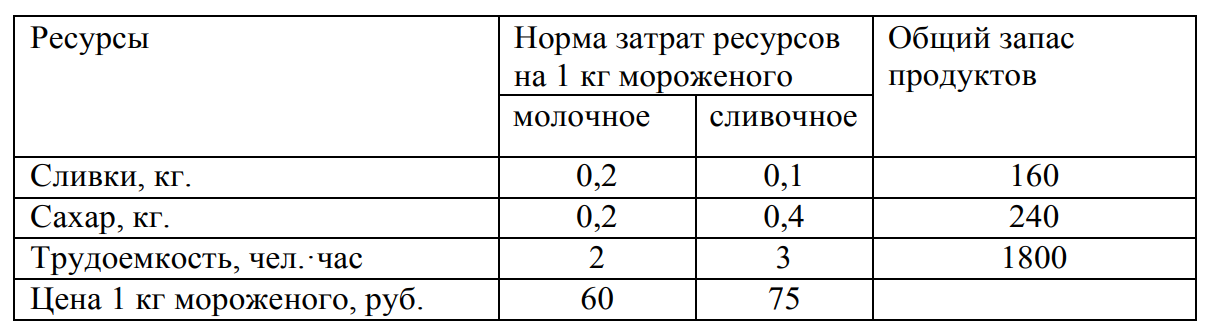
\includegraphics{image.png}
\caption{image.png}
\end{figure}

\begin{enumerate}
\def\labelenumi{\arabic{enumi}.}
\item
  Считая, что сбыт мороженого полностью обеспечен, определить, сколько
  сливочного и молочного мороженого должен выпускать в сутки комбинат,
  чтобы доход от реализации был максимальным.
\item
  Определить, увеличение запасов каких продуктов наиболее целесообразно
  и почему.
\item
  Если фонд рабочего времени снизится на 300 чел. час, как это повлияет
  на решение?
\item
  Если цена 1 кг молочного мороженого возрастет до 90 руб., как это
  повлияет на определение суточного плана производства?
\end{enumerate}

    \subsection{Построение математической
модели}\label{ux43fux43eux441ux442ux440ux43eux435ux43dux438ux435-ux43cux430ux442ux435ux43cux430ux442ux438ux447ux435ux441ux43aux43eux439-ux43cux43eux434ux435ux43bux438}

    \emph{Считая, что сбыт мороженого полностью обеспечен, определить,
сколько сливочного и молочного мороженого должен выпускать в сутки
комбинат, чтобы доход от реализации был максимальным.}

Для решения первого пункта составим математическую модель данной задачи.
Необходимо узнать, сколько килограмм сливочного и молочного мороженого
должен выпускать комбинат. Для типов мороженого введем соответствующие
переменные:

\begin{itemize}
\item
  \(x\) -- 1 кг молочного мороженого;
\item
  \(y\) -- 1 кг сливочного мороженого.
\end{itemize}

Нам необходимо максимизировать доход от продажи мороженого, при этом
вычислить, сколько килограмм для этого нужно продать. Математически это
можно сформулировать следующим образом: \[60x + 75y \to \max.\] То есть
функция \(z(x,y) = 60x+ 75y\) и будет являться целевой функцией.

Необходимо составить ограничения на производство. Их можно составить
непосредственно из таблицы, при этом учитывая, что килограммы не могут
быть отрицательны, то есть \(x, y\geq 0\). Таким образом, имеем задачу
линейного программирования \[z(x,y) = 60x + 75y \to \max.\]
\[\begin{cases}
0.2x + 0.1 y \leq 160,\\
0.2x + 0.4 y \leq 240,\\
2x+3y \leq 1800.
\end{cases}\] \[x,y \geq 0.\]

    \subsection{Программная реализация решения
задачи}\label{ux43fux440ux43eux433ux440ux430ux43cux43cux43dux430ux44f-ux440ux435ux430ux43bux438ux437ux430ux446ux438ux44f-ux440ux435ux448ux435ux43dux438ux44f-ux437ux430ux434ux430ux447ux438}

    Данаая задача решается на плоскости, поэтому для ее решения можно
использовать либо графический метод, либо симплекс метод.

Сперва приведем реализацию графического метода для данной задачи, где
пунктирными линиями мы обозначим линии уровня целевой функции.

    \begin{tcolorbox}[breakable, size=fbox, boxrule=1pt, pad at break*=1mm,colback=cellbackground, colframe=cellborder]
\prompt{In}{incolor}{18}{\boxspacing}
\begin{Verbatim}[commandchars=\\\{\}]
\PY{k+kn}{import} \PY{n+nn}{numpy} \PY{k}{as} \PY{n+nn}{np}
\PY{k+kn}{import} \PY{n+nn}{matplotlib}\PY{n+nn}{.}\PY{n+nn}{pyplot} \PY{k}{as} \PY{n+nn}{plt}

\PY{k}{def} \PY{n+nf}{plot\PYZus{}linear\PYZus{}programming\PYZus{}problem}\PY{p}{(}\PY{p}{)}\PY{p}{:}
    \PY{n}{x} \PY{o}{=} \PY{n}{np}\PY{o}{.}\PY{n}{linspace}\PY{p}{(}\PY{l+m+mi}{0}\PY{p}{,} \PY{l+m+mi}{1000}\PY{p}{,} \PY{l+m+mi}{1000}\PY{p}{)}
    \PY{n}{y1} \PY{o}{=} \PY{p}{(}\PY{l+m+mi}{160} \PY{o}{\PYZhy{}} \PY{l+m+mf}{0.2} \PY{o}{*} \PY{n}{x}\PY{p}{)} \PY{o}{/} \PY{l+m+mf}{0.1}
    \PY{n}{y2} \PY{o}{=} \PY{p}{(}\PY{l+m+mi}{240} \PY{o}{\PYZhy{}} \PY{l+m+mf}{0.2} \PY{o}{*} \PY{n}{x}\PY{p}{)} \PY{o}{/} \PY{l+m+mf}{0.4}
    \PY{n}{y3} \PY{o}{=} \PY{p}{(}\PY{l+m+mi}{1800} \PY{o}{\PYZhy{}} \PY{l+m+mi}{2} \PY{o}{*} \PY{n}{x}\PY{p}{)} \PY{o}{/} \PY{l+m+mi}{3}

    \PY{n}{z} \PY{o}{=} \PY{k}{lambda} \PY{n}{x}\PY{p}{,} \PY{n}{y}\PY{p}{:} \PY{l+m+mi}{60} \PY{o}{*} \PY{n}{x} \PY{o}{+} \PY{l+m+mi}{75} \PY{o}{*} \PY{n}{y}

    \PY{n}{fig}\PY{p}{,} \PY{n}{ax} \PY{o}{=} \PY{n}{plt}\PY{o}{.}\PY{n}{subplots}\PY{p}{(}\PY{p}{)}
    \PY{n}{ax}\PY{o}{.}\PY{n}{plot}\PY{p}{(}\PY{n}{x}\PY{p}{,} \PY{n}{y1}\PY{p}{,} \PY{n}{label}\PY{o}{=}\PY{l+s+s1}{\PYZsq{}}\PY{l+s+s1}{0.2x + 0.1y \PYZlt{}= 160}\PY{l+s+s1}{\PYZsq{}}\PY{p}{)}
    \PY{n}{ax}\PY{o}{.}\PY{n}{plot}\PY{p}{(}\PY{n}{x}\PY{p}{,} \PY{n}{y2}\PY{p}{,} \PY{n}{label}\PY{o}{=}\PY{l+s+s1}{\PYZsq{}}\PY{l+s+s1}{0.2x + 0.4y \PYZlt{}= 240}\PY{l+s+s1}{\PYZsq{}}\PY{p}{)}
    \PY{n}{ax}\PY{o}{.}\PY{n}{plot}\PY{p}{(}\PY{n}{x}\PY{p}{,} \PY{n}{y3}\PY{p}{,} \PY{n}{label}\PY{o}{=}\PY{l+s+s1}{\PYZsq{}}\PY{l+s+s1}{2x + 3y \PYZlt{}= 1800}\PY{l+s+s1}{\PYZsq{}}\PY{p}{)}
    \PY{n}{ax}\PY{o}{.}\PY{n}{set\PYZus{}xlim}\PY{p}{(}\PY{p}{(}\PY{l+m+mi}{0}\PY{p}{,} \PY{l+m+mi}{800}\PY{p}{)}\PY{p}{)}
    \PY{n}{ax}\PY{o}{.}\PY{n}{set\PYZus{}ylim}\PY{p}{(}\PY{p}{(}\PY{l+m+mi}{0}\PY{p}{,} \PY{l+m+mi}{800}\PY{p}{)}\PY{p}{)}
    \PY{n}{ax}\PY{o}{.}\PY{n}{set\PYZus{}xlabel}\PY{p}{(}\PY{l+s+s1}{\PYZsq{}}\PY{l+s+s1}{x}\PY{l+s+s1}{\PYZsq{}}\PY{p}{)}
    \PY{n}{ax}\PY{o}{.}\PY{n}{set\PYZus{}ylabel}\PY{p}{(}\PY{l+s+s1}{\PYZsq{}}\PY{l+s+s1}{y}\PY{l+s+s1}{\PYZsq{}}\PY{p}{)}
    \PY{n}{ax}\PY{o}{.}\PY{n}{set\PYZus{}title}\PY{p}{(}\PY{l+s+s1}{\PYZsq{}}\PY{l+s+s1}{Графическое представление задачи линейного программирования}\PY{l+s+s1}{\PYZsq{}}\PY{p}{)}

    \PY{n}{x\PYZus{}values} \PY{o}{=} \PY{n}{np}\PY{o}{.}\PY{n}{linspace}\PY{p}{(}\PY{l+m+mi}{0}\PY{p}{,} \PY{l+m+mi}{1000}\PY{p}{,} \PY{l+m+mi}{100}\PY{p}{)}
    \PY{n}{y\PYZus{}values} \PY{o}{=} \PY{n}{np}\PY{o}{.}\PY{n}{linspace}\PY{p}{(}\PY{l+m+mi}{0}\PY{p}{,} \PY{l+m+mi}{3000}\PY{p}{,} \PY{l+m+mi}{100}\PY{p}{)}
    \PY{n}{X}\PY{p}{,} \PY{n}{Y} \PY{o}{=} \PY{n}{np}\PY{o}{.}\PY{n}{meshgrid}\PY{p}{(}\PY{n}{x\PYZus{}values}\PY{p}{,} \PY{n}{y\PYZus{}values}\PY{p}{)}
    \PY{n}{Z} \PY{o}{=} \PY{n}{z}\PY{p}{(}\PY{n}{X}\PY{p}{,} \PY{n}{Y}\PY{p}{)}
    \PY{n}{ax}\PY{o}{.}\PY{n}{contour}\PY{p}{(}\PY{n}{X}\PY{p}{,} \PY{n}{Y}\PY{p}{,} \PY{n}{Z}\PY{p}{,} \PY{n}{levels}\PY{o}{=}\PY{l+m+mi}{20}\PY{p}{,} \PY{n}{colors}\PY{o}{=}\PY{l+s+s1}{\PYZsq{}}\PY{l+s+s1}{black}\PY{l+s+s1}{\PYZsq{}}\PY{p}{,} \PY{n}{alpha}\PY{o}{=}\PY{l+m+mf}{0.5}\PY{p}{,} \PY{n}{linestyles}\PY{o}{=}\PY{l+s+s1}{\PYZsq{}}\PY{l+s+s1}{dotted}\PY{l+s+s1}{\PYZsq{}}\PY{p}{)}

    \PY{n}{ax}\PY{o}{.}\PY{n}{legend}\PY{p}{(}\PY{p}{)}
    \PY{n}{ax}\PY{o}{.}\PY{n}{grid}\PY{p}{(}\PY{k+kc}{True}\PY{p}{)}

    \PY{n}{plt}\PY{o}{.}\PY{n}{show}\PY{p}{(}\PY{p}{)}

\PY{n}{plot\PYZus{}linear\PYZus{}programming\PYZus{}problem}\PY{p}{(}\PY{p}{)}
\end{Verbatim}
\end{tcolorbox}

    \begin{center}
    \adjustimage{max size={0.9\linewidth}{0.9\paperheight}}{output_6_0.png}
    \end{center}
    { \hspace*{\fill} \\}
    
    Таким образом, решением задачи является точка пересечения прямых
\(0.2x+0.1y = 160\) и \(0.2x + 0.4y = 240\). Из второго уравнения можно
вычесть первое и получить \[y=\dfrac{800}{3}.\] Тогда
\[x = \dfrac{2000}{3}.\] Отсюда оптимальное решение
\[(x^0, y^0) = \left(\dfrac{2000}3, \dfrac{80}3\right).\]

    Теперь построим решение задачи симплекс методом с помощью библиотеки
OR-Tools.

    \begin{tcolorbox}[breakable, size=fbox, boxrule=1pt, pad at break*=1mm,colback=cellbackground, colframe=cellborder]
\prompt{In}{incolor}{26}{\boxspacing}
\begin{Verbatim}[commandchars=\\\{\}]
\PY{c+c1}{\PYZsh{}pip install ortools}
\end{Verbatim}
\end{tcolorbox}

    \begin{tcolorbox}[breakable, size=fbox, boxrule=1pt, pad at break*=1mm,colback=cellbackground, colframe=cellborder]
\prompt{In}{incolor}{25}{\boxspacing}
\begin{Verbatim}[commandchars=\\\{\}]
\PY{k+kn}{from} \PY{n+nn}{ortools}\PY{n+nn}{.}\PY{n+nn}{linear\PYZus{}solver} \PY{k+kn}{import} \PY{n}{pywraplp}


\PY{k}{def} \PY{n+nf}{solve\PYZus{}lp\PYZus{}problem}\PY{p}{(}\PY{p}{)}\PY{p}{:}
    \PY{n}{solver} \PY{o}{=} \PY{n}{pywraplp}\PY{o}{.}\PY{n}{Solver}\PY{o}{.}\PY{n}{CreateSolver}\PY{p}{(}\PY{l+s+s2}{\PYZdq{}}\PY{l+s+s2}{GLOP}\PY{l+s+s2}{\PYZdq{}}\PY{p}{)}
    \PY{k}{if} \PY{o+ow}{not} \PY{n}{solver}\PY{p}{:}
        \PY{k}{return}

    \PY{n}{x} \PY{o}{=} \PY{n}{solver}\PY{o}{.}\PY{n}{NumVar}\PY{p}{(}\PY{l+m+mi}{0}\PY{p}{,} \PY{n}{solver}\PY{o}{.}\PY{n}{infinity}\PY{p}{(}\PY{p}{)}\PY{p}{,} \PY{l+s+s2}{\PYZdq{}}\PY{l+s+s2}{x}\PY{l+s+s2}{\PYZdq{}}\PY{p}{)}
    \PY{n}{y} \PY{o}{=} \PY{n}{solver}\PY{o}{.}\PY{n}{NumVar}\PY{p}{(}\PY{l+m+mi}{0}\PY{p}{,} \PY{n}{solver}\PY{o}{.}\PY{n}{infinity}\PY{p}{(}\PY{p}{)}\PY{p}{,} \PY{l+s+s2}{\PYZdq{}}\PY{l+s+s2}{y}\PY{l+s+s2}{\PYZdq{}}\PY{p}{)}
    
    \PY{n}{solver}\PY{o}{.}\PY{n}{Add}\PY{p}{(}\PY{l+m+mf}{0.2} \PY{o}{*} \PY{n}{x} \PY{o}{+} \PY{l+m+mf}{0.1} \PY{o}{*} \PY{n}{y} \PY{o}{\PYZlt{}}\PY{o}{=} \PY{l+m+mi}{160}\PY{p}{)}
    \PY{n}{solver}\PY{o}{.}\PY{n}{Add}\PY{p}{(}\PY{l+m+mf}{0.2} \PY{o}{*} \PY{n}{x} \PY{o}{+} \PY{l+m+mf}{0.4} \PY{o}{*} \PY{n}{y} \PY{o}{\PYZlt{}}\PY{o}{=} \PY{l+m+mi}{240}\PY{p}{)}
    \PY{n}{solver}\PY{o}{.}\PY{n}{Add}\PY{p}{(}\PY{l+m+mi}{2}\PY{o}{*} \PY{n}{x} \PY{o}{\PYZhy{}} \PY{l+m+mi}{3} \PY{o}{*} \PY{n}{y} \PY{o}{\PYZlt{}}\PY{o}{=} \PY{l+m+mi}{1800}\PY{p}{)}

    \PY{n}{solver}\PY{o}{.}\PY{n}{Maximize}\PY{p}{(}\PY{l+m+mi}{60} \PY{o}{*} \PY{n}{x} \PY{o}{+} \PY{l+m+mi}{75} \PY{o}{*} \PY{n}{y}\PY{p}{)}

    \PY{n+nb}{print}\PY{p}{(}\PY{l+s+sa}{f}\PY{l+s+s2}{\PYZdq{}}\PY{l+s+s2}{Solving with }\PY{l+s+si}{\PYZob{}}\PY{n}{solver}\PY{o}{.}\PY{n}{SolverVersion}\PY{p}{(}\PY{p}{)}\PY{l+s+si}{\PYZcb{}}\PY{l+s+s2}{\PYZdq{}}\PY{p}{)}
    \PY{n}{status} \PY{o}{=} \PY{n}{solver}\PY{o}{.}\PY{n}{Solve}\PY{p}{(}\PY{p}{)}

    \PY{k}{if} \PY{n}{status} \PY{o}{==} \PY{n}{pywraplp}\PY{o}{.}\PY{n}{Solver}\PY{o}{.}\PY{n}{OPTIMAL}\PY{p}{:}
        \PY{n+nb}{print}\PY{p}{(}\PY{l+s+s2}{\PYZdq{}}\PY{l+s+s2}{Solution:}\PY{l+s+s2}{\PYZdq{}}\PY{p}{)}
        \PY{n+nb}{print}\PY{p}{(}\PY{l+s+sa}{f}\PY{l+s+s2}{\PYZdq{}}\PY{l+s+s2}{Objective value = }\PY{l+s+si}{\PYZob{}}\PY{n}{solver}\PY{o}{.}\PY{n}{Objective}\PY{p}{(}\PY{p}{)}\PY{o}{.}\PY{n}{Value}\PY{p}{(}\PY{p}{)}\PY{l+s+si}{\PYZcb{}}\PY{l+s+s2}{\PYZdq{}}\PY{p}{)}
        \PY{n+nb}{print}\PY{p}{(}\PY{l+s+sa}{f}\PY{l+s+s2}{\PYZdq{}}\PY{l+s+s2}{x = }\PY{l+s+si}{\PYZob{}}\PY{n}{x}\PY{o}{.}\PY{n}{solution\PYZus{}value}\PY{p}{(}\PY{p}{)}\PY{l+s+si}{\PYZcb{}}\PY{l+s+s2}{\PYZdq{}}\PY{p}{)}
        \PY{n+nb}{print}\PY{p}{(}\PY{l+s+sa}{f}\PY{l+s+s2}{\PYZdq{}}\PY{l+s+s2}{y = }\PY{l+s+si}{\PYZob{}}\PY{n}{y}\PY{o}{.}\PY{n}{solution\PYZus{}value}\PY{p}{(}\PY{p}{)}\PY{l+s+si}{\PYZcb{}}\PY{l+s+s2}{\PYZdq{}}\PY{p}{)}
    \PY{k}{else}\PY{p}{:}
        \PY{n+nb}{print}\PY{p}{(}\PY{l+s+s2}{\PYZdq{}}\PY{l+s+s2}{The problem does not have an optimal solution.}\PY{l+s+s2}{\PYZdq{}}\PY{p}{)}

    \PY{n+nb}{print}\PY{p}{(}\PY{l+s+sa}{f}\PY{l+s+s2}{\PYZdq{}}\PY{l+s+s2}{Problem solved in }\PY{l+s+si}{\PYZob{}}\PY{n}{solver}\PY{o}{.}\PY{n}{iterations}\PY{p}{(}\PY{p}{)}\PY{l+s+si}{:}\PY{l+s+s2}{d}\PY{l+s+si}{\PYZcb{}}\PY{l+s+s2}{ iterations}\PY{l+s+s2}{\PYZdq{}}\PY{p}{)}


\PY{n}{solve\PYZus{}lp\PYZus{}problem}\PY{p}{(}\PY{p}{)}
\end{Verbatim}
\end{tcolorbox}

    \begin{Verbatim}[commandchars=\\\{\}]
Solving with Glop solver v9.9.3963
Solution:
Objective value = 60000.0
x = 666.6666666666667
y = 266.6666666666666
Problem solved in 2 iterations
    \end{Verbatim}

    В итоге получили идентичное решение. Также мы выяснили, что значение
целевой функции в оптимальной токчке равно \[z(x^0, y^0)=60000.\]

    \emph{Определить, увеличение запасов каких продуктов наиболее
целесообразно и почему.}

Для определения наиболее целесообразного увеличения запасов продуктов,
нужно проанализировать ограничения модели. В данном случае, увеличение
запасов сливок или сахара будет целесообразным, если соответствующие
ограничения станут более жесткими. То есть, если при увеличении запасов
на единицу, значение соответствующего ограничения увеличится, то это
будет иметь положительный эффект на максимизацию дохода.

    \emph{Если фонд рабочего времени снизится на 300 чел. час, как это
повлияет на решение?}

Для ответа на этот вопрос необходимо изменить соответствующие
ограничения в задаче линейного программирования. В частности мы изменим
3 ограничение, считая теперь, что у нас трудоемкость 1500 чел/час.

Таким образом, имеем задачу линейного программирования
\[z(x,y) = 60x + 75y \to \max.\] \[\begin{cases}
0.2x + 0.1 y \leq 160,\\
0.2x + 0.4 y \leq 240,\\
2x+3y \leq 1500.
\end{cases}\] \[x,y \geq 0.\]

    \begin{tcolorbox}[breakable, size=fbox, boxrule=1pt, pad at break*=1mm,colback=cellbackground, colframe=cellborder]
\prompt{In}{incolor}{28}{\boxspacing}
\begin{Verbatim}[commandchars=\\\{\}]
\PY{k}{def} \PY{n+nf}{solve\PYZus{}lp\PYZus{}problem\PYZus{}1}\PY{p}{(}\PY{p}{)}\PY{p}{:}
    \PY{n}{solver} \PY{o}{=} \PY{n}{pywraplp}\PY{o}{.}\PY{n}{Solver}\PY{o}{.}\PY{n}{CreateSolver}\PY{p}{(}\PY{l+s+s2}{\PYZdq{}}\PY{l+s+s2}{GLOP}\PY{l+s+s2}{\PYZdq{}}\PY{p}{)}
    \PY{k}{if} \PY{o+ow}{not} \PY{n}{solver}\PY{p}{:}
        \PY{k}{return}

    \PY{n}{x} \PY{o}{=} \PY{n}{solver}\PY{o}{.}\PY{n}{NumVar}\PY{p}{(}\PY{l+m+mi}{0}\PY{p}{,} \PY{n}{solver}\PY{o}{.}\PY{n}{infinity}\PY{p}{(}\PY{p}{)}\PY{p}{,} \PY{l+s+s2}{\PYZdq{}}\PY{l+s+s2}{x}\PY{l+s+s2}{\PYZdq{}}\PY{p}{)}
    \PY{n}{y} \PY{o}{=} \PY{n}{solver}\PY{o}{.}\PY{n}{NumVar}\PY{p}{(}\PY{l+m+mi}{0}\PY{p}{,} \PY{n}{solver}\PY{o}{.}\PY{n}{infinity}\PY{p}{(}\PY{p}{)}\PY{p}{,} \PY{l+s+s2}{\PYZdq{}}\PY{l+s+s2}{y}\PY{l+s+s2}{\PYZdq{}}\PY{p}{)}
    
    \PY{n}{solver}\PY{o}{.}\PY{n}{Add}\PY{p}{(}\PY{l+m+mf}{0.2} \PY{o}{*} \PY{n}{x} \PY{o}{+} \PY{l+m+mf}{0.1} \PY{o}{*} \PY{n}{y} \PY{o}{\PYZlt{}}\PY{o}{=} \PY{l+m+mi}{160}\PY{p}{)}
    \PY{n}{solver}\PY{o}{.}\PY{n}{Add}\PY{p}{(}\PY{l+m+mf}{0.2} \PY{o}{*} \PY{n}{x} \PY{o}{+} \PY{l+m+mf}{0.4} \PY{o}{*} \PY{n}{y} \PY{o}{\PYZlt{}}\PY{o}{=} \PY{l+m+mi}{240}\PY{p}{)}
    \PY{n}{solver}\PY{o}{.}\PY{n}{Add}\PY{p}{(}\PY{l+m+mi}{2}\PY{o}{*} \PY{n}{x} \PY{o}{\PYZhy{}} \PY{l+m+mi}{3} \PY{o}{*} \PY{n}{y} \PY{o}{\PYZlt{}}\PY{o}{=} \PY{l+m+mi}{1500}\PY{p}{)}

    \PY{n}{solver}\PY{o}{.}\PY{n}{Maximize}\PY{p}{(}\PY{l+m+mi}{60} \PY{o}{*} \PY{n}{x} \PY{o}{+} \PY{l+m+mi}{75} \PY{o}{*} \PY{n}{y}\PY{p}{)}

    \PY{n+nb}{print}\PY{p}{(}\PY{l+s+sa}{f}\PY{l+s+s2}{\PYZdq{}}\PY{l+s+s2}{Solving with }\PY{l+s+si}{\PYZob{}}\PY{n}{solver}\PY{o}{.}\PY{n}{SolverVersion}\PY{p}{(}\PY{p}{)}\PY{l+s+si}{\PYZcb{}}\PY{l+s+s2}{\PYZdq{}}\PY{p}{)}
    \PY{n}{status} \PY{o}{=} \PY{n}{solver}\PY{o}{.}\PY{n}{Solve}\PY{p}{(}\PY{p}{)}

    \PY{k}{if} \PY{n}{status} \PY{o}{==} \PY{n}{pywraplp}\PY{o}{.}\PY{n}{Solver}\PY{o}{.}\PY{n}{OPTIMAL}\PY{p}{:}
        \PY{n+nb}{print}\PY{p}{(}\PY{l+s+s2}{\PYZdq{}}\PY{l+s+s2}{Solution:}\PY{l+s+s2}{\PYZdq{}}\PY{p}{)}
        \PY{n+nb}{print}\PY{p}{(}\PY{l+s+sa}{f}\PY{l+s+s2}{\PYZdq{}}\PY{l+s+s2}{Objective value = }\PY{l+s+si}{\PYZob{}}\PY{n}{solver}\PY{o}{.}\PY{n}{Objective}\PY{p}{(}\PY{p}{)}\PY{o}{.}\PY{n}{Value}\PY{p}{(}\PY{p}{)}\PY{l+s+si}{\PYZcb{}}\PY{l+s+s2}{\PYZdq{}}\PY{p}{)}
        \PY{n+nb}{print}\PY{p}{(}\PY{l+s+sa}{f}\PY{l+s+s2}{\PYZdq{}}\PY{l+s+s2}{x = }\PY{l+s+si}{\PYZob{}}\PY{n}{x}\PY{o}{.}\PY{n}{solution\PYZus{}value}\PY{p}{(}\PY{p}{)}\PY{l+s+si}{\PYZcb{}}\PY{l+s+s2}{\PYZdq{}}\PY{p}{)}
        \PY{n+nb}{print}\PY{p}{(}\PY{l+s+sa}{f}\PY{l+s+s2}{\PYZdq{}}\PY{l+s+s2}{y = }\PY{l+s+si}{\PYZob{}}\PY{n}{y}\PY{o}{.}\PY{n}{solution\PYZus{}value}\PY{p}{(}\PY{p}{)}\PY{l+s+si}{\PYZcb{}}\PY{l+s+s2}{\PYZdq{}}\PY{p}{)}
    \PY{k}{else}\PY{p}{:}
        \PY{n+nb}{print}\PY{p}{(}\PY{l+s+s2}{\PYZdq{}}\PY{l+s+s2}{The problem does not have an optimal solution.}\PY{l+s+s2}{\PYZdq{}}\PY{p}{)}

    \PY{n+nb}{print}\PY{p}{(}\PY{l+s+sa}{f}\PY{l+s+s2}{\PYZdq{}}\PY{l+s+s2}{Problem solved in }\PY{l+s+si}{\PYZob{}}\PY{n}{solver}\PY{o}{.}\PY{n}{iterations}\PY{p}{(}\PY{p}{)}\PY{l+s+si}{:}\PY{l+s+s2}{d}\PY{l+s+si}{\PYZcb{}}\PY{l+s+s2}{ iterations}\PY{l+s+s2}{\PYZdq{}}\PY{p}{)}


\PY{n}{solve\PYZus{}lp\PYZus{}problem\PYZus{}1}\PY{p}{(}\PY{p}{)}
\end{Verbatim}
\end{tcolorbox}

    \begin{Verbatim}[commandchars=\\\{\}]
Solving with Glop solver v9.9.3963
Solution:
Objective value = 60000.0
x = 666.6666666666666
y = 266.66666666666663
Problem solved in 3 iterations
    \end{Verbatim}

    Как можно заметить, данное нововведение никак не повлияло на результат
решения задачи линейного программирования.

    \emph{Если цена 1 кг молочного мороженого возрастет до 90 руб., как это
повлияет на определение суточного плана производства?}

Для решения этой задачи мы изменим целевую функцию, учитывая новую цену
за килограмм молочного мороженого. Таким образом, задача линейного
программирования будет получена следующая:
\[z(x,y) = 90x + 75y \to \max.\] \[\begin{cases}
0.2x + 0.1 y \leq 160,\\
0.2x + 0.4 y \leq 240,\\
2x+3y \leq 1800.
\end{cases}\] \[x,y \geq 0.\]

    \begin{tcolorbox}[breakable, size=fbox, boxrule=1pt, pad at break*=1mm,colback=cellbackground, colframe=cellborder]
\prompt{In}{incolor}{29}{\boxspacing}
\begin{Verbatim}[commandchars=\\\{\}]
\PY{k}{def} \PY{n+nf}{solve\PYZus{}lp\PYZus{}problem\PYZus{}1}\PY{p}{(}\PY{p}{)}\PY{p}{:}
    \PY{n}{solver} \PY{o}{=} \PY{n}{pywraplp}\PY{o}{.}\PY{n}{Solver}\PY{o}{.}\PY{n}{CreateSolver}\PY{p}{(}\PY{l+s+s2}{\PYZdq{}}\PY{l+s+s2}{GLOP}\PY{l+s+s2}{\PYZdq{}}\PY{p}{)}
    \PY{k}{if} \PY{o+ow}{not} \PY{n}{solver}\PY{p}{:}
        \PY{k}{return}

    \PY{n}{x} \PY{o}{=} \PY{n}{solver}\PY{o}{.}\PY{n}{NumVar}\PY{p}{(}\PY{l+m+mi}{0}\PY{p}{,} \PY{n}{solver}\PY{o}{.}\PY{n}{infinity}\PY{p}{(}\PY{p}{)}\PY{p}{,} \PY{l+s+s2}{\PYZdq{}}\PY{l+s+s2}{x}\PY{l+s+s2}{\PYZdq{}}\PY{p}{)}
    \PY{n}{y} \PY{o}{=} \PY{n}{solver}\PY{o}{.}\PY{n}{NumVar}\PY{p}{(}\PY{l+m+mi}{0}\PY{p}{,} \PY{n}{solver}\PY{o}{.}\PY{n}{infinity}\PY{p}{(}\PY{p}{)}\PY{p}{,} \PY{l+s+s2}{\PYZdq{}}\PY{l+s+s2}{y}\PY{l+s+s2}{\PYZdq{}}\PY{p}{)}
    
    \PY{n}{solver}\PY{o}{.}\PY{n}{Add}\PY{p}{(}\PY{l+m+mf}{0.2} \PY{o}{*} \PY{n}{x} \PY{o}{+} \PY{l+m+mf}{0.1} \PY{o}{*} \PY{n}{y} \PY{o}{\PYZlt{}}\PY{o}{=} \PY{l+m+mi}{160}\PY{p}{)}
    \PY{n}{solver}\PY{o}{.}\PY{n}{Add}\PY{p}{(}\PY{l+m+mf}{0.2} \PY{o}{*} \PY{n}{x} \PY{o}{+} \PY{l+m+mf}{0.4} \PY{o}{*} \PY{n}{y} \PY{o}{\PYZlt{}}\PY{o}{=} \PY{l+m+mi}{240}\PY{p}{)}
    \PY{n}{solver}\PY{o}{.}\PY{n}{Add}\PY{p}{(}\PY{l+m+mi}{2}\PY{o}{*} \PY{n}{x} \PY{o}{\PYZhy{}} \PY{l+m+mi}{3} \PY{o}{*} \PY{n}{y} \PY{o}{\PYZlt{}}\PY{o}{=} \PY{l+m+mi}{1800}\PY{p}{)}

    \PY{n}{solver}\PY{o}{.}\PY{n}{Maximize}\PY{p}{(}\PY{l+m+mi}{90} \PY{o}{*} \PY{n}{x} \PY{o}{+} \PY{l+m+mi}{75} \PY{o}{*} \PY{n}{y}\PY{p}{)}

    \PY{n+nb}{print}\PY{p}{(}\PY{l+s+sa}{f}\PY{l+s+s2}{\PYZdq{}}\PY{l+s+s2}{Solving with }\PY{l+s+si}{\PYZob{}}\PY{n}{solver}\PY{o}{.}\PY{n}{SolverVersion}\PY{p}{(}\PY{p}{)}\PY{l+s+si}{\PYZcb{}}\PY{l+s+s2}{\PYZdq{}}\PY{p}{)}
    \PY{n}{status} \PY{o}{=} \PY{n}{solver}\PY{o}{.}\PY{n}{Solve}\PY{p}{(}\PY{p}{)}

    \PY{k}{if} \PY{n}{status} \PY{o}{==} \PY{n}{pywraplp}\PY{o}{.}\PY{n}{Solver}\PY{o}{.}\PY{n}{OPTIMAL}\PY{p}{:}
        \PY{n+nb}{print}\PY{p}{(}\PY{l+s+s2}{\PYZdq{}}\PY{l+s+s2}{Solution:}\PY{l+s+s2}{\PYZdq{}}\PY{p}{)}
        \PY{n+nb}{print}\PY{p}{(}\PY{l+s+sa}{f}\PY{l+s+s2}{\PYZdq{}}\PY{l+s+s2}{Objective value = }\PY{l+s+si}{\PYZob{}}\PY{n}{solver}\PY{o}{.}\PY{n}{Objective}\PY{p}{(}\PY{p}{)}\PY{o}{.}\PY{n}{Value}\PY{p}{(}\PY{p}{)}\PY{l+s+si}{\PYZcb{}}\PY{l+s+s2}{\PYZdq{}}\PY{p}{)}
        \PY{n+nb}{print}\PY{p}{(}\PY{l+s+sa}{f}\PY{l+s+s2}{\PYZdq{}}\PY{l+s+s2}{x = }\PY{l+s+si}{\PYZob{}}\PY{n}{x}\PY{o}{.}\PY{n}{solution\PYZus{}value}\PY{p}{(}\PY{p}{)}\PY{l+s+si}{\PYZcb{}}\PY{l+s+s2}{\PYZdq{}}\PY{p}{)}
        \PY{n+nb}{print}\PY{p}{(}\PY{l+s+sa}{f}\PY{l+s+s2}{\PYZdq{}}\PY{l+s+s2}{y = }\PY{l+s+si}{\PYZob{}}\PY{n}{y}\PY{o}{.}\PY{n}{solution\PYZus{}value}\PY{p}{(}\PY{p}{)}\PY{l+s+si}{\PYZcb{}}\PY{l+s+s2}{\PYZdq{}}\PY{p}{)}
    \PY{k}{else}\PY{p}{:}
        \PY{n+nb}{print}\PY{p}{(}\PY{l+s+s2}{\PYZdq{}}\PY{l+s+s2}{The problem does not have an optimal solution.}\PY{l+s+s2}{\PYZdq{}}\PY{p}{)}

    \PY{n+nb}{print}\PY{p}{(}\PY{l+s+sa}{f}\PY{l+s+s2}{\PYZdq{}}\PY{l+s+s2}{Problem solved in }\PY{l+s+si}{\PYZob{}}\PY{n}{solver}\PY{o}{.}\PY{n}{iterations}\PY{p}{(}\PY{p}{)}\PY{l+s+si}{:}\PY{l+s+s2}{d}\PY{l+s+si}{\PYZcb{}}\PY{l+s+s2}{ iterations}\PY{l+s+s2}{\PYZdq{}}\PY{p}{)}


\PY{n}{solve\PYZus{}lp\PYZus{}problem\PYZus{}1}\PY{p}{(}\PY{p}{)}
\end{Verbatim}
\end{tcolorbox}

    \begin{Verbatim}[commandchars=\\\{\}]
Solving with Glop solver v9.9.3963
Solution:
Objective value = 80000.0
x = 666.6666666666667
y = 266.6666666666666
Problem solved in 2 iterations
    \end{Verbatim}

    Как можно увидеть, данное нововведение повлияло лишь на значение целевой
функции в ее точке максимума. Оптимальное решение же осталось
неизменным.


    % Add a bibliography block to the postdoc
    
    
    
\end{document}
